The first step in the design process is to understand the domain of the API. It helps to identify required
input parameters, return values, and types expressed in the domain language.
It is also important to capture possible API evolution in the future, so the modeled API is flexible enough
to support it without drastic changes and breaking backwards compatibility.

There are 3 types of the IGMPv2 messages - Membership Query, Membership Report, and Leave Group message.
All types of messages follow the same format of the packet header but with different values in the fields.
The structure of the IGMPv2 packet is depicted in the Figure~\ref{fig:igmp_packet}.

\begin{figure}[!htb]
\centering
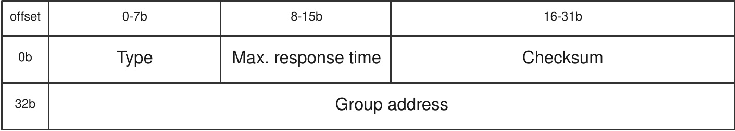
\includegraphics[width=1.0
\textwidth]{igmp_packet}
\caption{Structure of the IGMPv2 packet}
\label{fig:igmp_packet}
\end{figure}

From the perspective of the API design, there are following key differences between constructed types of packets:

\begin{enumerate}
    \item Membership Query - Type field is set to 0x11 value.
    Both maximum response time and group address can have non-zero value.
    In case of General Query, group address is set to \textit{0.0.0.0} value (all multicast groups are queries
    in the broadcast domain).
    In case of Group-Specific Query, group address should contain valid multicast address that is queried by router.
    \item Membership Report - Type field is set to 0x12 value.
    Maximum response time is always set to 0 (unused).
    Group address should contain valid multicast address reported by client.
    \item Leave Group - Type field is set to 0x17 value.
    Maximum response time is always set to 0 (unused).
    Group address should contain valid multicast address that client wants to leave.
\end{enumerate}

The following list summarizes the findings from the domain analysis which we have to keep in mind during
the design process:

\begin{itemize}
    \item There are 3 types of the IGMPv2 messages that differ in the constant values of the fields.
    Serialization logic, that will be implemented as the business logic, is common for all types of messages.
    \item There are 2 configurable parameters (aside from the type of message) that client should be able to specify
    on the input - maximum response time and group address.
    However, there are some constraints on the values of these parameters based on the type
    of the IGMPv2 message (for example, Leave Group message maximum response time is always set to 0)
    and field length (number of bytes).
    \item API should not contain any return type since serialized data will be written to the output stream
    (for example, backed by network socket) that is passed as the input parameter.
    \item In the future client may require to support also IGMPv1 and IGMPv3 protocols.
    Especially IGMPv3 protocol specify additional fields in the packet header that are not present
    in the IGMPv2 protocol.
    There is also open room for possible support of IPv6 flavour of the IGMP protocol
    - Multicast Listener Discovery (MLD) that is implemented by the Internet Group Management Protocol (IGMP).
\end{itemize}
